\cotefile{14}
\scanpage{74}
% @1 heading
Relations entre $\underline{\mathrm{Alb}}_X^0$, $\underline{\mathrm{Pic}}_X^{00}$ et $H^1(X)$, $H^{2n-1}(X)$
% @2 hypothesis
($X$ projective lisse conn. de dim $n$ sur $k$ alg. clos).
% @3 first relation
\[
 \pi_1^\ell(\underline{\mathrm{Alb}}_X^0)
 \xleftarrow{\overset{(t)}{\sim}}\pi_1^{\ell}(X)^{\mathrm{ab}}(\ell)
 \deleted{\unsure{\simeq}}\inserted{\unsure{\xleftarrow{\overset{(t)}{\sim}}|\overset{(t)}{\simeq}}H^{2n-1}(X)(n)}
 \qquad \{\text{à \uline{torsion près}}\}\quad
 [\text{c'est tjrs surjectif ?}]
\]
% @4–5 second relation
\[
 \pi_1(\underline{\mathrm{Pic}}_X^{00})\simeq H^1(\underline{\mathrm{Alb}}_X^0)(1)
 \xrightarrow{\overset{t}{\sim}}H^1(X)(1)
 \qquad \begin{aligned}&\text{\uline{à torsion près}}\\&[\text{c'est tjrs injectif \deleted{\unsure{?|!}}}]\end{aligned}
\]
% @6 third relation
\[
 H^1(\underline{\mathrm{Alb}}_X^0)\xrightarrow{\overset{t}{\sim}}H^1(X)
 \qquad \text{\uline{à torsion près}}\quad [\text{c'est tjrs injectif \deleted{\unsure{?|!}}}]
\]
% @7 fourth relation
\[
 H^1(\underline{\mathrm{Pic}}_X^{00})\simeq\pi_1(\underline{\mathrm{Alb}}_X)(-1)
 \xleftarrow{\overset{(t)}{\sim}}H^{2n-1}(X)(n-1)
 \qquad\text{\deleted{\unsure{[c'est|c'est} tjrs}}
\]

% @8 sentence
Si on \unsure{représ.|représ|repère} les VA par les $H^1$,
% @9–10 brace
\diagram{$\left\{\begin{array}{lll}
 \underline{\mathrm{Alb}}_X & \text{correspond à} & H^1(X)\\
 \underline{\mathrm{Pic}}_X\, . & \rule{3cm}{0.35pt} & H^{2n-1}(X)(n-1)
\end{array}\right.$}
% archive sheet number: 73

\scanpage{75}
% @0 top centre
\mspage{7}
% @1–3 opening
More specifically, let $A=K[t]={}$ the polynomial ring in one indeterminate $t$, and let us determine the possible $\uuline{A}$-cogroup structures on $A$. Let $m:A\to A\otimes A$ be defined
% @4–6 formula and first axiom
by $m(t)=\displaystyle\sum_{i,j}\alpha_{ij}t^i\otimes t^j$ ($\alpha_{ij}\in K$). Without losing generality, we assume that $e_A:A\to A$ is given by $e_A(t)=0$. Then, the dual of $5\handwritten{^\circ}$ is satisfied if we let $e_F:A\to K$ be given by
% @7–11 axioms and coassociativity
$e_F(t)=0$. Require that $(A,m)$ satisfy the dual of $2\handwritten{^\circ}\mathrm L$ and $2\handwritten{^\circ}\mathrm R$, and we conclude readily that $m(t)=t\otimes1+1\otimes t+{}+\sum\nolimits_{i>0,\,j>0}\alpha_{ij}t^i\otimes t^j$. Next, require $m$ to satisfy the dualized $1\handwritten{^\circ}$ (the associativity); simple calculation shows that
% @12–13 first display
\[
\begin{aligned}
 &m(t)\otimes1+1\otimes1\otimes t+\sum\nolimits_{i>0,\,j>0}\alpha_{ij}m(t)^i\otimes t^j={}\\
 &{}=t\otimes1\otimes1+1\otimes m(t)+\sum\nolimits_{i>0,\,j>0}\handwritten{\alpha_{ij}}t^i\otimes m(t)^j,\quad\text{or}
\end{aligned}
\]
% @14–15 numbered display
\begingroup\makeatletter\tagsleft@true\makeatother
\[
\begin{aligned}[t]
 &\sum\alpha_{ij}(t^i\otimes t^j\otimes1)+\sum\alpha_{ij}(m(t)^i\otimes t^j)={}\\
 &{}=\sum\alpha_{ij}(1\otimes t^i\otimes t^j)+\sum\alpha_{ij}(t^i\otimes m(t)^j)
\end{aligned}\tag*{(3.1)}
\]
\endgroup
% @16–19 largest indices
must hold. Suppose that $\alpha_{pq},\ldots,\alpha_{pr}$ are the non-zero members of the set $\{\alpha_{ij}\}_{\substack{i>0\\j>0}}$ with the largest first index $p$. Among $\alpha_{pq},\ldots,\alpha_{pr}$ suppose $\alpha_{pq}$ to have the largest second index $q$. Then, the left-hand side of (3.1) yields a term
% @20–23 leading term
$\alpha_{pq}\alpha_{pq}^p(t^p\otimes t^q)^p\otimes t^q$, which cannot be cancelled out by any other term unless $p=1$. Therefore, $p=\max\{i;\alpha_{ij}\ne0\}=1$, or else $\alpha_{ij}=0$ for $i>0$, $j>0$. Likewise one proves that $\max\{j;\alpha_{ij}\ne0\}=1$ or all $\alpha_{ij}=0$. Consequently,
% archive sheet number: 74

\scanpage{76}
% @1–2 top
\textcircled{I} \textcircled{1} VA catégorie \inserted{additive} définie \deleted{\unsure{à l'aide|à isog. près}} \deleted{sur}\inserted{par} un corps alg. clos $k$
% @3 duality
\[
 \mathrm{VA}^{\unsure{o|0|\circ}}\xrightarrow{*}\mathrm{VA}\qquad
 A\mathrel{\unsure{\sim|\leadsto}}A^* \qquad\text{foncteur \deleted{\unsure{dualisant}}\inserted{``dualité''}}
\]
% @4–7 graded rings
\[
 \mathrm{VA}^{o}\xrightarrow{C^*}
 \left(\begin{gathered}\text{Anneaux}\\ \text{gradués comm.,}\\
 \text{à degrés }\geqslant 0,\end{gathered}\right)
 \qquad \begin{gathered} A\sim C^*\quad\text{cycles}\\\text{mod équiv.}\\\text{alg.}\end{gathered}
\]
\[
 \deleted{\unsure{A}}C^0\simeq\mathbb Z
\]
% @8 dimension
Fonction dimension, additive, invariante par dualité.

% @9–11 point 2
\textcircled{2}
\[
\begin{aligned}
 C^n(A)&\mathrel{\deleted{\unsure{\leftarrow}}}
 \xrightarrow{\overset{\deleted{\unsure{n|\int_x|\deg}}\unsure{\chi|X}}{\sim}}\mathbb Z
 &&\text{isom can, mais pas fonctoriel}\\
 &&&\quad\text{\unsure{sauf pr|fonct. pour} isom.}\\
 C^0(A)&\xleftarrow{\sim}\mathbb Z &&\text{isom fonctoriel}
\end{aligned}
\]
% @12–14 projection
Loi \uline{covariante} pour les cycles, formule de projection (contenant la formule de transposition)

% @15–16 Pontrjagin
On peut en tirer formellement la loi de \unsure{Pontriagin|Pontrjagin} pour les cycles \ldots.

% @17–19 point 3
\textcircled{3} Application fondamentale
\diagram{\begin{tikzcd}[ampersand replacement=\&,column sep=small,row sep=small]
 C^1(A)\arrow[rr]\arrow[dr,dashed] \& \& \operatorname{Hom}(A,A^*)^{\mathrm{alt}}\\
 \& \deleted{\unsure{\mathrm{Pic}}}C^1(A\times A)\arrow[ur,dashed] \&
\end{tikzcd}}
% @19 lower left boxed
\margin{\fbox{\parbox{\dimexpr\marginparwidth-2\fboxsep-2\fboxrule\relax}{N.B. On pourrait définir \unsure{axiomatiqmt|axiomatiquement} $A^*$ par cette formule}}}
% @20–21 lower right
ou au choix
\diagram{\begin{tikzcd}[ampersand replacement=\&,row sep=tiny]
 \& \bigl(\text{\unsure{isom|isom.}}\quad C^1(A\times B)/C^1(A)\times C^1(B)\bigr)\\
 C^1(A\times B)\arrow[r] \& \operatorname{Hom}(A,B^*)\arrow[u,phantom,"\rotatebox{90}{$\simeq$}" description]
\end{tikzcd}}
% archive sheet number: 75

\scanpage{77}
% @0 upper right
\mspage{- 20 -}
% @1–4 continuation
cribles $R\handwritten{\hookrightarrow}X$ couvrant $X$. La deuxième suite spectrale s'en déduit immédiatement et peut d'ailleurs s'interpréter comme une suite spectrale de foncteurs composés (formule (17)). Les assertions sur les morphismes $\handwritten{\Phi}^q$ et $\handwritten{\Phi}^q_X$ s'obtiennent en remarquant que les termes
% @5 display
\[
 \handwritten{\check{\mathscr H}}^0(\handwritten{\mathscr H}^q(F))\qquad q\ne0
\]
% @6 nullity
sont nuls ((2.2) et (formule (23)).

% @7–11 bracketed corollary
\noindent\begin{tikzpicture}
\node[inner sep=3pt] (cor) {\begin{minipage}{.89\linewidth}
\uline{Corollaire 2.6} : (au corollaire 2.5) : Soient $E$ un topos, $A$ un \handwritten{A}nneau de $E$ (commutatif à élément unité), $S$ un objet de $E$, $F$ un $A$-Module. Désignons par $\underline F$ le groupe abélien sous-jacent à $F$. Le foncteur $F\handwritten{\leadsto}\underline F$ est exact et par suite l'isomorphisme canonique :
% @12 degree zero
\[
 H^0(E/S,F)\mathrel{\overset{\handwritten{\sim}}{\relbar\joinrel\handwritten{\rightarrow}}}H^0(E.S,\underline F)
\]
% @13 introduction
définit des morphismes :
% @14 degree q
\[
 H^q(E/S,F)\mathrel{\relbar\joinrel\handwritten{\rightarrow}}H^q(E/S,\underline F)
\]
% @15 conclusion
Ces morphismes sont des isomorphismes.
\end{minipage}};
\handwritten{\draw (cor.north west) ++(2pt,1pt) -- (cor.north west) -- (cor.south west) -- ++(2pt,-1pt);}
\end{tikzpicture}

% @16–19 proof
\uline{Preuve} : On se ramène immédiatement au cas où $E$ est une catégorie de faisceaux sur un site $C\handwritten{\in \underline U}$ dont $S$ est un objet (2.4.14.II). On peut aussi (3.\handwritten{5}.4.III) supposer que les produits fibrés sont représentables dans $C$.
% @20 encircled typed phrase
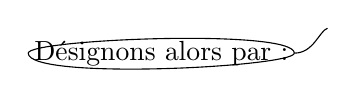
\begin{tikzpicture}[baseline=(phrase.base)]
\node[inner sep=2pt] (phrase) {Désignons alors par :};
\handwritten{\draw[thin] (phrase.east) .. controls +(7pt,0pt) and +(-3pt,-1pt) .. ++(12pt,9pt);
\draw[thin] (phrase.east) .. controls +(0,9pt) and +(0,5pt) .. (phrase.west) .. controls +(0,-10pt) and +(0,-5pt) .. (phrase.east);}
\end{tikzpicture}
% @21 final display
\[
 \handwritten{\mathscr H}^0:\ C_A^{\handwritten{\sim}}\mathrel{\relbar\joinrel\handwritten{\rightarrow}} C_A^{\wedge}
\]
% @22 foot
\hfill \ldots/\ldots
% archive sheet number: 76

\scanpage{78}
% @1–2 first bracket
\textcircled{1}
\noindent\(\left[\vcenter{\hbox{\begin{minipage}{.92\linewidth}\footnotesize
\[
\begin{aligned}
 \mathrm{VA}^{\deleted{\unsure{o|*}}}
 &\xrightarrow{T^{\deleted{\unsure{Q_\ell}}}_{\unsure{\mathbb Q|Q}_\ell}}
 \mathrm{Mod}(\mathbb Q_\ell)
 & A&\leadsto\deleted{\unsure{H}}T_\ell(A)\otimes_{\mathbb Z_\ell}\mathbb Q_\ell\\
 \mathrm{VA}^{\unsure{o|0|\circ}}
 &\xrightarrow{H^1_\ell}\mathrm{Mod}(\mathbb Q_\ell)
 & A&\mathrel{\unsure{\sim|\leadsto}} H^1(A,\mathbb Q_\ell)
 =\operatorname{Hom}_{\deleted{\unsure{\mathbb Z_\ell}}}(T_{\mathbb Q_\ell}(A),\mathbb Q_\ell)
\end{aligned}
\]
% @3 qualification
foncteurs \uline{fidèles}, \uline{additifs}
% @4 exterior algebra
\[
 H^*(A)=\bigwedge\nolimits^* H^1(A)
\]
% @5–8 square
\diagram{\begin{tikzcd}[ampersand replacement=\&,row sep=large,column sep=large]
 \deleted{\unsure{A}}\mathrm{VA}^o \arrow[r,"*"]\arrow[d,"(H^1)^o"] \& \mathrm{VA}\arrow[d,"H^1"]
 \& A\sim A^*\arrow[d,phantom,"\text{(\unsure{équivalence|équivalences})}" description]\\
 {\mathrm{Mod}\,\mathbb Q_\ell}^{o}\arrow[r,"{\operatorname{Hom}(\cdot,\mathbb Q_\ell(-1))}"'] \& \mathrm{Mod}\,\mathbb Q_\ell \& \text{carré comm. à \unsure{isom|sens|isom.} près.}
\end{tikzcd}}

\end{minipage}}}\right.\)

% @9 cancelled start
$\deleted{\unsure{Z^i(A)\longrightarrow}}$
% @10–12 second bracket
\margin{\unsure{1|4}}
\noindent\(\left[\vcenter{\hbox{\begin{minipage}{.92\linewidth}\footnotesize
\[
 \mathrm{VA}\xrightarrow{\deleted{Z}C^*}(\mathrm{Ab})\qquad
 A\sim\deleted{Z}C^*(A)
\]
\inserted{anneau de Chow (ou cycles mod \uline{équiv. alg})}
% @13–15 class map
\diagram{\begin{tikzcd}[ampersand replacement=\&,column sep=small,row sep=small]
 \deleted{Z}C^i\arrow[r] \& H^{2i}\otimes\mathbb Q_\ell(i)\arrow[d,phantom,"\rotatebox{90}{$=$}" description]
 \& \deleted{Z}C^i(A)\arrow[r,"{\gamma_A^{2i}}"] \& H^{\unsure{2i|i}}(A,\mathbb Q_\ell)(i)\\
 \& \bigwedge^{2i}H^1\otimes\mathbb Q_\ell(i) \& \& \text{compatible avec}
\end{tikzcd}}
\hfill structure d'anneau,
\end{minipage}}}\right.\)

% @16–20 third bracket
2
\noindent\(\left[\vcenter{\hbox{\begin{minipage}{.92\linewidth}\footnotesize
\diagram{\begin{tikzcd}[ampersand replacement=\&,column sep=small,row sep=tiny]
 H^{2n}(A)\arrow[r,phantom,"\simeq" description] \& \bigwedge^{2n}H^1(A)\arrow[r,"{\unsure{\eta|\int}_A}","\sim" description] \& \mathbb Q_\ell(-n) \& \text{\uline{isom \unsure{canonique|canoniques}}}\\
 \& \times \& \times \&\\
 H^{2n}(A^*)\arrow[r,phantom,"\simeq" description] \& \bigwedge^{2n}H^1(A^*)\arrow[d,phantom,"\wr" description]\arrow[r,phantom,"\simeq" description,"{\eta_{A^*}}"'] \& \mathbb Q_\ell(-n)\arrow[d,phantom,"\wr" description,"{\text{\textcircled{\scriptsize can.}}}"] \& \text{id}\\
 \& \mathbb Q_\ell(\unsure{+2n|-2n|2n}) \& \mathbb Q_\ell(-2n) \& \text{vérifier s'il n'y a pas}\\
 \& \& \& \text{un signe !}
\end{tikzcd}}
\end{minipage}}}\right.\)
% archive sheet number: 77

\scanpage{79}
% @0 upper right
\mspage{- 25 -}
% @1–2 continuation bracket
\noindent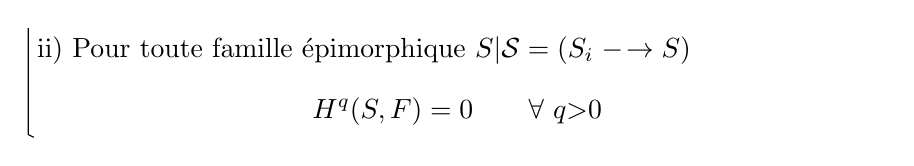
\begin{tikzpicture}
\node[inner sep=3pt] (ii) {\begin{minipage}{.88\linewidth}
ii) Pour toute famille épimorphique $\handwritten{\unsure{\mathscr S|\mathcal S}}=(S_i\mathrel{\relbar\joinrel\handwritten{\rightarrow}}S)$
\[
 H^q(\handwritten{\mathscr S},F)=0\qquad \handwritten{\forall}\ q\handwritten{>}0
\]
\end{minipage}};
\handwritten{\draw (ii.north west) -- (ii.south west) -- ++(2pt,-1pt);}
\end{tikzpicture}

% @3–4 forward implication
\uline{Preuve} : (i) $\handwritten{\Longrightarrow}$ (ii). Se déduit immédiatement de la suite exacte de la proposition 1.5

% @5–6 converse
(ii) $\handwritten{\Longrightarrow}$ (i). Soit $S$ un objet de $E$. Il existe une sous-catégorie pleine $C$ de $E$ qui possède les propriétés suivantes :

% @7–8 clause a
a) L'ensemble des objets de $C$ peut être indexé par un élément de l'univers et est une famille de générateurs de $E$.

% @9 clause b
b) Les produits fibrés sont représentables dans $C$.

% @10 clause c
\tikz[baseline=(cc.base)]{\node[inner sep=1pt] (cc) {c)};\handwritten{\draw (cc.north east) ++(-1pt,3pt) -- ++(0,-3pt) .. controls +(-16pt,2pt) and +(-14pt,-5pt) .. (cc.south east) -- ++(0,-2pt);}} L'objet $S$ est un objet de $C$.

% @11–14 topology
Munissons alors $C$ de la topologie induite par $E$. La catégorie des faisceaux d'ensembles sur $C$ est équivalente à $E$ (3.5.4.III). Le faisceau $F$ induit alors sur $C$ un faisceau $C$-acyclique ((3.1) et (1.6)) par suite :
% @15 vanishing
\[
 H^q(S,F)=0\qquad\handwritten{\forall}\ q\handwritten{>}0
\]
% @16 closing
\hfill c.q.f.d.

% @17–21 definition bracket
\noindent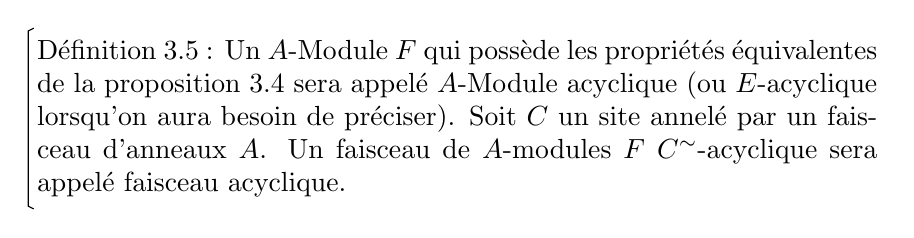
\begin{tikzpicture}
\node[inner sep=3pt] (defn) {\begin{minipage}{.88\linewidth}
\uline{Définition 3.5} : Un $A$-Module $F$ qui possède les propriétés équivalentes de la proposition 3.4 sera appelé $A$-Module \uline{acyclique} (ou $E$-acyclique lorsqu'on aura besoin de préciser). Soit $C$ un site annelé par un faisceau d'anneaux $A$. Un faisceau de $A$-modules $F$ $C^{\handwritten{\sim}}$-acyclique sera appelé faisceau \uline{acyclique}.
\end{minipage}};
\handwritten{\draw (defn.north west) ++(2pt,1pt) -- (defn.north west) -- (defn.south west) -- ++(2pt,-1pt);}
\end{tikzpicture}
% @22 foot
\hfill \ldots/\ldots
% archive sheet number: 78

\scanpage{80}
% @1 first line and interline
3) Soit $u:A'\longrightarrow A$ une \deleted{isogénie}\inserted{\unsure{isom|hom|homom.}, avec $\dim A\unsure{.|-|=}\dim A'=n$}, alors
% @2–4 top-degree comparison
\diagram{\begin{tikzcd}[ampersand replacement=\&,column sep=small,row sep=small]
 u^{2n}: \& H^{2n}(A)\arrow[r]\arrow[d,phantom,"\rotatebox{90}{$\simeq$}" description] \& H^{2n}(A')\arrow[d,phantom,"\rotatebox{90}{$\simeq$}" description] \& \text{est donné par}\\
 \& \unsure{\mathbb Q|Q}_\ell(-n) \& \mathbb Q_\ell(-n) \&
\end{tikzcd}}
% @5–6 degree
la multiplication par $\deg u=d$ (nul ssi $u(A')\ne A$, i.e. $u$ n'est pas une isogénie).

% @7–8 transpose
En d'autres termes, définissant $u_*$
\[
 u_*:\ H^{*}(A)\mathrel{-}H^{\unsure{*|1}}(A')
\]
% @9–10 proviso
par transposition (Attention, à l'hyp que $A$ et $A'$ ont \unsure{=|même} dim) on trouve
% @11 unit
\[
 u_0(1_A)=d.1_{A'}
\]
% @12–13 arbitrary dimensions
Supposons que \deleted{les} \deleted{degrés} dim $n,n'$ de $A,A'$ soient quelconques, on définit par transposition
% @14 shifted map
\[
 H^i(A)\longrightarrow H^{i+2(n'-n)}(A')(n'-n)
\]
% @15–16 crossed opening
\deleted{et on va} qui se déduit \unsure{directmt|directement} de la connaissance de
% @17–18 pullback
\[
 u^1:\ H^1(A')\longrightarrow H^1(A)
 \qquad\left(\begin{gathered}\text{d'où }u^*:H^*(A')\to H^*(A)\\ \text{par }\bigwedge\nolimits^*\end{gathered}\right)
\]
% @19–20 last lines
et des isom $\unsure{\eta|\int}_A$ et $\eta_{A'}$, par transposition.

\unsure{Noter|Notons} que
% archive sheet number: 79

\scanpage{81}
% @1 cancelled opening
$\deleted{\unsure{H^0}}$
% @2 opening class
\[
 u_0(1_A)\in H^{\unsure{2|1}(n'-n)}(A')(n'-n)
\]
% @3–5 image cycle
est la classe du cycle image $u(A)\in\deleted{Z}C^{n'-n}(A)$ (de façon \unsure{général|générale}, $u_*$ compatible avec les op. \unsure{analogues} sur les cycles \ldots), donc
% @6–9 dimension cases
est nulle si $u(A)$ est de dim $<n$, et si $u(A)$ est de dim $n$, et si $B$ désigne la V.A. \deleted{\unsure{sa|son|sous}} image (au sens faisceautique) et $d$ le degré de projection $A\to B$,
% @10–12 image of the unit
alors $u_*(1_A)$ est égal à
\diagram{\begin{tikzcd}[ampersand replacement=\&,row sep=small]
 \deleted{\unsure{a|d}}d\,\gamma_{A'}^{2(n'-n)}(B)\arrow[d]\\
 \text{classe de}\\[-1ex]\text{Coh. associée}
\end{tikzcd}}

% @13–15 transpose
En termes de $H^1(A'^{\deleted{\unsure{*}}})\to H^1(A)$ : on regarde \unsure{le transposé|la transposée} (à val. dans $\unsure{\mathbb Q|Q}_\ell\deleted{\unsure{(-1)}}$)
$u_1:T_{\mathbb Q_\ell}(A)\longrightarrow T_{\mathbb Q_\ell}(A')$, \deleted{on prend} s'il n'est pas
% @16–19 injectivity
injectif on trouve $0$, s'il est injectif on trouve un multivecteur \deleted{dual de}\inserted{de degré} $2(n'-n)=\dim\operatorname{Coker}u_1$, qui définit une forme $2(n'-n)$-fois \unsure{lin.|lin}\ alternée sur $T_{\mathbb Q_\ell}(A')$
% archive sheet number: 80

\scanpage{82}
% @0 upper right
\mspage{- 23 -}
% @1–2 underlying sheaf
La propriété de $C$-acyclicité ne dépend que du faisceau abélien sous-jacent (2.6).

% @3–5 restriction
Soient $C$ et $C'$ deux sites et $u:C\mathrel{\relbar\joinrel\handwritten{\rightarrow}}C'$ un foncteur continu (3.2.2.III). Il n'est pas vrai, en général, que la restriction à $C''$ d'un faisceau $C'$-acyclique soit $C$-acyclique.

% @6–7 proposition
\noindent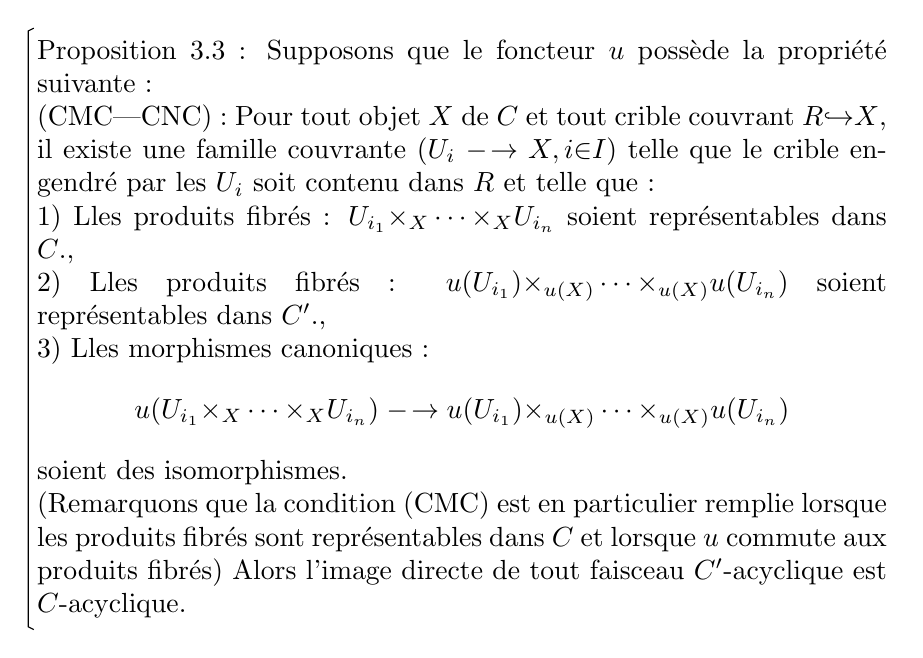
\begin{tikzpicture}
\node[inner sep=3pt] (prop) {\begin{minipage}{.89\linewidth}
\uline{Proposition 3.3} : Supposons que le foncteur $u$ possède la propriété suivante :

% @8–10 covering condition
(\unsure{CMC|CNC}) : Pour tout objet $X$ de $C$ et tout crible couvrant $R\handwritten{\hookrightarrow}X$, il existe une famille couvrante $(U_i\mathrel{\relbar\joinrel\handwritten{\rightarrow}}X,i\handwritten{\in} I)$ tel\handwritten{le} que le crible engendré par les $U_i$ soit contenu dans $R$ et telle que :

% @11–12 first product
1) \deleted{L}\handwritten{l}e\handwritten{s} produits fibrés : $U_{i_1}\handwritten{\times}_X\cdots\handwritten{\times}_X U_{i_n}$ soient représentables dans $C$\deleted{.}\handwritten{,}

% @13–14 second product
2) \deleted{L}\handwritten{l}es produits fibrés : $u(U_{i_1})\handwritten{\times}_{u(X)}\cdots\handwritten{\times}_{u(X)}u(U_{i_n})$ soient représentables dans $C'$\deleted{.}\handwritten{,}

% @15–17 morphisms
3) \deleted{L}\handwritten{l}es morphismes canoniques :
\[
 u(U_{i_1}\handwritten{\times}_X\cdots\handwritten{\times}_X U_{i_n})\mathrel{\relbar\joinrel\handwritten{\rightarrow}}
 u(U_{i_1})\handwritten{\times}_{u(X)}\cdots\handwritten{\times}_{u(X)}u(U_{i_n})
\]
soient des isomorphismes.

% @18–21 conclusion
(Remarquons que la condition (CMC) est en particulier remplie lorsque les produits fibrés sont représentables dans $C$ et lorsque $u$ commute aux produits fibrés) Alors l'image directe de tout faisceau $C'$-acyclique est $C$-acyclique.
\end{minipage}};
\handwritten{\draw (prop.north west) ++(2pt,1pt) -- (prop.north west) -- (prop.south west) -- ++(2pt,-1pt);}
\end{tikzpicture}
% @22 foot
\hfill \ldots/\ldots
% archive sheet number: 81

\scanpage{83}
% @1–2 continuation
nulle sur $\unsure{\mathbb Q|Q}_\ell(A)$ (ce qui \unsure{la|le} \unsure{caractérise|choisir} \unsure{à|:} un scalaire près) et tel que, si
% @3 exact sequence
\[
 \unsure{0|\cdot}\mathrel{\unsure{-|\to}}K\mathrel{-}H^1(A'^{\deleted{\unsure{*}}})\longrightarrow H^1(A)\mathrel{-}0
 \qquad\text{\unsure{l'isom|l'isomt|l'isom.|1ère}}
\]
% @4–6 determinant comparison
\diagram{\begin{tikzcd}[ampersand replacement=\&,column sep=small,row sep=small]
 \bigwedge^{2n'}H^1(A'^{\deleted{\unsure{*}}})\arrow[d,phantom,"\rotatebox{90}{$\simeq$}" description]\arrow[r,phantom,"\simeq" description]
 \& \deleted{\unsure{H}}\bigwedge^{2n}H^1(A)\arrow[d,phantom,"\rotatebox{90}{$\simeq$}" description] \& {}\otimes\deleted{\unsure{H}}\bigwedge^{2(n'-n)}K\\
 H^{2n'}(A'), \& H^{2n}(A) \&
\end{tikzcd}}
% @7–10 characteristic classes
\deleted{\unsure{à}} la classe caractéristique de $H^{2n}(A)(n)$ fois la classe \unsure{cherchée|duale} $u_*(1_A)$ de $\bigwedge^{2(n'-n)}K(n'-n)$ corresponde \uline{$d$ fois} la classe caractéristique de $H^{2n'}(A')(n')$. \uline{N.B.} $d$ est aussi le
% @11 integral lattices
contenu de $T_{\text{\textcircled{$\scriptstyle\mathbb Z_\ell$}}}(A)$ dans $T_{\text{\textcircled{$\scriptstyle\mathbb Z_\ell$}}}(A')$.

% @12–14 duality
\[
 H^i(A)\times H^{2n-i}(A)\longrightarrow H^{2n}(A)\simeq\mathbb Q_\ell(-n)
\]
est une dualité, donc
\[
 H^i(A)\simeq H^{2n-i}(A)'(-n)\simeq\bigwedge^{2n-i}T_{\mathbb Q_\ell}(A)(-n)
\]
% @15–17 transpose square
\deleted{En particulier,} Ceci posé, l'hom $\deleted{u_*}$
\diagram{\begin{tikzcd}[ampersand replacement=\&,column sep=small,row sep=small]
 u_*: \& H^i(A)\arrow[r]\arrow[d,phantom,"\rotatebox{90}{$\simeq$}" description] \& H^{i+\deleted{\unsure{2n}}2(n'-n)}(A')(n'-n)\\
 \& \deleted{\unsure{H}}\bigwedge^{2n-i}T_{\mathbb Q_\ell}(A)(-n)\arrow[r] \& \bigwedge^{2n-i}T_{\mathbb Q_\ell}(A')(-n)
\end{tikzcd}}
% @18 bottom edge
s'identifie : $\bigwedge^{2n-1}u_1\deleted{\otimes}\otimes\mathbb Q_\ell(-n)$.
% archive sheet number: 82

\scanpage{84}
% @0 upper right
\mspage{- 22 -}
% @1–2 proposition
\noindent\begin{tikzpicture}
\node[inner sep=3pt] (prop) {\begin{minipage}{.89\linewidth}
\uline{Proposition 3.1} : Soient $C$ un site annelé et $\unsure{G|C}$ un faisceau d\handwritten{e} $A$-modules sur $C$. Les conditions suivantes sont équivalentes :

% @3–4 condition i
i) Pour tout objet $X$ de $C$ et tout crible couvrant $R\handwritten{\hookrightarrow}X$
\[
 H^q(C^{\wedge}/R,\handwritten{\mathscr H}^0(G))=0\qquad\handwritten{\forall}\ q\handwritten{>}0
\]
% @5–6 condition ii
ii) Pour tout objet $X$ de $C$
\[
 \handwritten{\check}{H}^q(C^{\wedge}/X,\handwritten{\mathscr H}^0(G))=0\qquad\handwritten{\forall}\ q\handwritten{>}0
\]
% @7 ii bis
ii)$^{\mathrm{bis}}$ Les préfaisceaux $\handwritten{\check{\mathscr H}}^q\,\handwritten{\mathscr H}^0(G)$ sont nuls pour tout $q\handwritten{>}0$.

% @8–9 condition iii
iii) Pour tout objet $X$ de $C$
\[
 H^q(C^{\handwritten{\sim}}/X,G)=0\qquad\handwritten{\forall}\ q\handwritten{>}0
\]
% @10 iii bis
iii)$^{\mathrm{bis}}$ Les préfaisceaux $\handwritten{\mathscr H}^q(G)$ sont nuls pour tout $q\handwritten{>}0$.
\end{minipage}};
\handwritten{\draw (prop.north west) ++(2pt,1pt) -- (prop.north west) -- (prop.south west) -- ++(2pt,-1pt);}
\end{tikzpicture}

% @11–17 proof
\uline{Preuve} : Il est clair qu'on a les équivalences $(\mathrm{ii})\handwritten{\Longleftrightarrow}(\mathrm{ii})^{\mathrm{bis}}$ (N$^\circ$ 2, formules (14) et (15)) et $(\mathrm{iii})\handwritten{\Longleftrightarrow}(\mathrm{iii})^{\mathrm{bis}}$ (N$^\circ$ 2, formule (12)). D'autre part, on a l'implication $(\mathrm{i})\handwritten{\Longrightarrow}(\mathrm{ii})$ \handwritten{(}N$^\circ$ 2, formule (14)) et l'implication $(\mathrm{iii})^{\mathrm{bis}}\handwritten{\Longrightarrow}(\mathrm{i})$ par la suite spectrale de la proposition 2.3 Il nous reste donc à montrer l'implication $(\mathrm{ii})^{\mathrm{bis}}\handwritten{\Longrightarrow}(\mathrm{iii})^{\mathrm{bis}}$ qui résulte immédiatement de la dernière assertion de (2.5) c.q.f.d.

% @18–20 definition
\noindent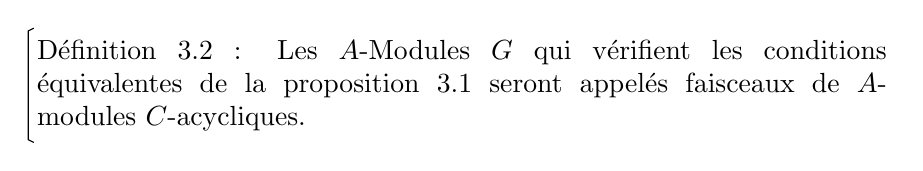
\begin{tikzpicture}
\node[inner sep=3pt] (defn) {\begin{minipage}{.89\linewidth}
\uline{Définition 3.2} : Les $A$-Modules $G$ qui vérifient les conditions équivalentes de la proposition 3.1 seront appelés faisceaux de $A$-modules \uline{$C$-acycliques}.
\end{minipage}};
\handwritten{\draw (defn.north west) ++(2pt,1pt) -- (defn.north west) -- (defn.south west) -- ++(2pt,-1pt);}
\end{tikzpicture}
% @21 foot
\hfill \ldots/\ldots
% archive sheet number: 83

\scanpage{85}
% @1–3 exterior class and compressed interline
De cette façon, on retrouve $u_*(1_A)$ où $1_A\in H^0(A)=(\deleted{\unsure{H}}\bigwedge^{2n}T_{\unsure{\mathbb Q|Q}_\ell}\deleted{A}(A))\deleted{\unsure{\otimes}}(-n)$, \deleted{à partir}\inserted{$u_*(\unsure{1_A|A})\in\bigwedge^{2n}T_{\mathbb Q_\ell}(\unsure{A'|A})(-n)$} de $u_1:T_{\mathbb Q_\ell}(A)\mathrel{-}T_{\mathbb Q_\ell}(A')$, en prenant
% @4 exterior map
\[
 \bigwedge^{2n}u_1\otimes\mathbb Q_\ell(-\unsure{n|1})\deleted{\unsure{)}}:
 \bigwedge^{2n}T_{\mathbb Q_\ell}(A)(-n)\longrightarrow\bigwedge^{2n}T_{\mathbb Q_\ell}(A')(-n)
\]
% @5–6 image
en prenant l'Image de la classe fondamentale du premier \unsure{mb|mbr}. \(/\!/\) On voit ainsi
% @7–9 final assertion
que \deleted{si $u$ est \unsure{i}} la connaissance de $u_{\unsure{*|0}}(1)$ détermine l'image de $u_1:T_\ell(A)\mathrel{-}T_\ell(A')$, dans le cas où cet hom est injectif.
% archive sheet number: 84

\scanpage{86}
% @0 upper right
\mspage{- 21 -}
% @1 opening
le foncteur d'injection et par :
% @2 functor
\[
 \handwritten{\underline{\mathscr H}}^0:C_{\mathrm{Ab}}^{\handwritten{\sim}}\mathrel{\relbar\joinrel\handwritten{\rightarrow}}C_{\mathrm{Ab}}^{\wedge}
\]
% @3–7 reduction; the two pencil lines connect ends to following starts
le foncteur d'injection pour les faisceaux abéliens.\tikz[remember picture,baseline]\coordinate (aend);\par
\noindent\tikz[remember picture,baseline]\coordinate (bstart);
Il suffit évidemment de montrer que si $F$ est un $A$-Module acyclique pour $\handwritten{\mathscr H}^0$, alors $\underline F$ est acyclique pour $\handwritten{\underline{\mathscr H}}^0$.\tikz[remember picture,baseline]\coordinate (bend);\par
\noindent\tikz[remember picture,baseline]\coordinate (cstart);
Soit donc $F$ un $A$-Module $\handwritten{\mathscr H}^0$-acyclique. Le corollaire (2.5) montre alors que pour tout objet $X$ de $C$ :
\begin{tikzpicture}[remember picture,overlay]
\handwritten{\draw[thin] (aend) .. controls +(3pt,-6pt) and +(-4pt,6pt) .. (bstart);}
\handwritten{\draw[thin] (bend) .. controls +(3pt,-6pt) and +(-4pt,6pt) .. (cstart);}
\end{tikzpicture}
% @8 module cohomology
\[
 \handwritten{\check}{H}^q(X,\handwritten{\mathscr H}^0(F))=0\qquad(0\handwritten{<}q)
\]
% @9–11 first parenthesis and reference
(\deleted{L}\handwritten{l}e foncteur dérivé étant calculé ici dans la catégorie des préfaisceaux de $A$-modules)

La proposition (1.5) et la formule (15) montre\handwritten{nt} alors que :
% @12 underlying group
\[
 \handwritten{\check}{H}^q(X,\handwritten{\mathscr H}^0(\underline F))=0\qquad(0\handwritten{<}q)
\]
% @13–15 second parenthesis and reference
(\deleted{L}\handwritten{l}e foncteur dérivé étant calculé ici dans la catégorie des préfaisceaux abéliens)

Le corollaire (2.5) montre alors que :
% @16–17 last display
\[
 \handwritten{\mathscr H}^q(\underline F)=0\qquad(0\handwritten{<}q)
\]
\hfill c.q.\handwritten{f}.d.

% @18 heading
\begin{center}\uline{N$^\circ$ 3. Critères d'acyclicité}\end{center}

% @19–20 announcement
Nous allons définir une première famille de faisceaux acycliques.
% @21 foot
\hfill \ldots/\ldots
% archive sheet number: 85

